\pagebreak %sI will take those out later, for now they will help me to write

\section{Baumslag-Solitar groups and their generalisation}

In this chapter we will explore a certain class of groups, which were initially introduced in \cite{BaSo62}. They have since served as examples and counterexamples of groups with different properties.

\subsection{Definition and first properties}

\begin{definition}
    A \emph{Baumslag-Solitar group $BS(m,n)$} is a group given by the presentation \[BS(m,n) = \langle \: a, t\:|\:t(a^m)t^{-1} = a^n \: \rangle \] where $m,n \in \Z \setminus \{0\}$.
\end{definition}

\begin{remark}
    Note, that for $m = n = 1$, $BS(m,n) = \langle a,t \: | \: tat^{-1} = a \: \rangle \cong \Z \times \Z$. This case seems to be regarded as somehow seperate in the literature.
\end{remark}

The first property of these groups that we will consider, and the one that motivated Baumslag and Solitar in \cite{BaSo62}, is that of being (non-)Hopfian.

\begin{definition}
    A group $G$ is said to be \emph{Hopfian} if every epimorphism from $G$ to itself is injective. In other words, if $G/N \cong G$ implies $N = 1$. Otherwise, we say $G$ is \emph{non-Hopfian}.
\end{definition}
    
Before we proceed, we should mention that examples of Hopfian groups include:
\begin{enumerate}
    \item simple groups;
    \item $(\mathbb{Q},+)$;
    \item finitely generated residually finite groups (by the theorem of Mal'cev), where we say that $G$ is residualy finite if for each $g \neq 1_G$ in $G$, there exists a finite group $F$ and a group homomorphism $\phi: G \to F$ such that $\phi(g) \neq 1_F$.
    \item finitely generated free groups.
\end{enumerate}

Examples (1) - (3) were taken from \cite{CeSi23}. An interested reader can find proofs of (3) and (4) being Hopfian in \cite[~chapters I, IV]{LySch15}. 

\begin{importantexample}\cite[page 514]{BrHa11}
    The group $BS(2,3) = \langle a,t \: | \: t(a^2)t^{-1} = a^3\rangle $ is non-Hopfian. To see that, one considers $\phi: BS(2,3) \to BS(2,3)$ defined on generators as $a \mapsto a^2$, and $t \mapsto t$. Note, that $a = a^3a^{-2} = ta^2t^{-1}a^{-2}$, so $a$ is in the image of $\phi$. Therefore, $\phi$ is onto, but also $[a,tat^{-1}] = atat^{-1}a^{-1}ta^{-1}t^{-1}$ is mapped to identity by $\phi$, thus being an example of a nontrivial element in $ker(\phi)$.
\end{importantexample}

\textcolor{red}{maybe add more properties?}

\subsubsection{Baumslag-Solitar groups as HNN extensions}

In this subsection we will follow the definitions and conventions from \cite[pages 497-498]{BrHa11}.

\begin{definition}
\label{HNN}
    Let $G$ be a group, $\phi: A_1 \to A_2$ an isomorphism between two subgroups $A_1$,$A_2$ of $G$. A \emph{HNN extension of G} associated to that data is the quotient of $G \ast \langle t \rangle$ by the smallest normal subgroup containing $\{a^{-1}t\phi(a)t^{-1} \: | \: a \in A_1 \}$. Thus, we can represent that extension by a relative presentation 
    \[G \ast_\phi = ( G,t \: | \: t^{-1}at = \phi(a), \forall a \in A_1). \]
\end{definition}

\begin{remark}
    If $A$ is an abstract group isomorphic to both $A_1$, $A_2$, then instead of $G \ast _\phi$ we may write $G \ast _A$. We refer to $G \ast _A$ as a 'HNN extension of $G$ over $A$'.
\end{remark}

\begin{example}\label{BS as HNN}
    $BS(m,n)$ is a HNN extension of $\Z  =\langle b \rangle$. To see this, we consider two subgroups of $\Z$, $m\Z = \{b^{mk}\: | \: k \in \Z\}$ and $n\Z = \{b^{nk}\: | \: k \in \Z\}$ with $m,n \in \Z \setminus \{0\}$. Note, that we are using multiplicative notation for the ease of the later argument, so $b^m$ means ``\emph{add $b$ to itself $m$ times}. Define $\phi: m\Z \to n\Z$, by $b^{mk} \mapsto b^{nk}$. Then, $\phi$ is an isomorphism, and we can consider $\Z\ast_\phi = (\Z,t \: | \: t^{-1}at = \phi(a), \forall a\in m\Z)$. It is not hard to see though, that because $\Z = \langle b \rangle$, $\Z\ast_\phi = ( b,t \: | \: t^{-1}((b^k)^m)t = \phi((b^k)^m), \: \forall b^k\in \Z ) = \langle b,t \: | \: t^{-1}(b^m)t = b^n\rangle $, which is exactly the presentation of $BS(m,n)$.
\end{example}

%One of the reasons that HNN extensions are important is because together with free products with amalgamation they form the building blocks of graphs of groups (in the sense of Bass and Serre).

\subsection{Graphs of groups and $G$-trees}
%plan for this section - define G-trees and maybe how they connect to graphs of groups;
%you should definitely try to work out how the BS trees abd graphs would look like  -  maybe try to look through trees by Serre

For the discussion in this subsection we will follow \cite[chapter I]{Ser80}.

\begin{definition}
    A \emph{graph} $\Gamma$ consists of 
    \begin{itemize}
        \item a set $X = \:vert\:\Gamma$,
        \item a set $Y = \:edge\:\Gamma$,
        \item $Y \to  X \times X$ with $ y \mapsto (o(y), t(y))$, and 
        \item $Y \to Y$ with $y \mapsto \overline{y}$
    \end{itemize}
     which satisfy the following condition: for each $y \in Y$ we have $\overline{\overline{y}} = y$, $\overline{y} \neq y$ and $o(y) = t(\overline{y})$.
\end{definition}

We call elements of $X$ \emph{vertices}, and elements of $Y$ \emph{(oriented) edges}. Given $y \in Y$, the edge $\overline{y}$ is said to be the \emph{inverse edge}. Note, that we can define a morphism of graphs by mapping vertices to vertices, and mapping an edge between two vertices to an edge between their images.

Another notion that we can associate to a graph $\Gamma$ is that of orientation. That is, an \emph{orientation} of $\Gamma$ is a subset $Y_+$ of $Y$ such that $Y$ is a disjoint union of $Y_+$ and $\overline{Y_+}$. We can then define, up to isomorphism, an \emph{oriented graph}, by giving the two sets $X$ and $Y_+$ with a map $Y_+ \to X \times X$. The set of edges $Y$ is the disjoint union we described before.

%Using the concept of the oriented graph, we are able to define the following.

%\begin{definition}
%    Let $G$ be a group, $S$ a subset of $G$. Let $\Gamma(G,S)$ denote the oriented graph which has $G$ as its vertices, $(G \times S) = (edge\: \Gamma)_+$ as its orientation with $o(g,s) = g$ and $t(g,s) = gs$ for each edge $(g,s) \in G \times S$.
%\end{definition}

%Note that the action of $G$ by left multiplication on $\Gamma(G,S)$ preserves orientation and is free on both vertices and edges.

We are almost ready to define trees, which is a class of graphs that will be important later. The only thing we need, is the definition of a circuit.

\begin{definition}
    For an integer $n \ge 1$, $Circ_n$ is an oriented graph with $X = \{0,1, \ldots , n-1 \}$ and edges $Y_+ = \{ y \:| \: (o(y),(t(y)) = (i,i+1), \: i\in \{0,1,\ldots,n-1\} $ where $(n-1, (n-1) + 1)$ is set to $(n-1,0)\}$. A \emph{circuit} (of length $n$) in a graph is any subgraph isomorphic to $Circ_n$.
\end{definition}

\begin{definition} 
    A tree is a connected non-empty graph with no circuits.
\end{definition}

\begin{definition}\label{grpgraph}
    A graph of groups $(G,T)$ consists of a graph $T$, a group $G_p$ for each $p \in vert\:T$, and a group $G_y$ for each $y \in edge\: T$, together with a monomorphism $G_y \to G_{t(y)}$ (denoted $a \mapsto a^y$). In addition, it is required that $G_y = G_{\overline{y}}$.
\end{definition}

If in the above definition $T$ is a tree, then we call $(G,T)$ a tree of groups.

Another notion is one of a $G$-tree. We will connect it to the concept of a tree of groups at the end of this subsection.

\begin{definition}
    Let $G$ be a group, and $X$ a graph on which it acts. An \emph{inversion} is a pair $g \in G$, $y$ edge of $X$, such that $gy = \overline{y}$. If there is no such pair, we say that $G$ acts \emph{without inversion}. 
\end{definition}

Note, that saying that $G$ acts without inversion on $X$ is exactly the same as saying that the $G$-action preserves the orientation of $X$.

\begin{definition}
    A $G$-tree is a tree on which the group $G$ acts by automorphisms, without inversion.
\end{definition}

\begin{definition}
    For a graph of groups $(G,Y)$, the group $F(G,Y)$ is generated by groups $G_p$ and the elements $y \in Y$ subject to relations $\overline{y} = y^{-1}$ and $ya^yy^{-1} = a^{\overline{y}}$ if $y \in edge \: Y$, $a \in G_y$.
\end{definition}

A more precise way to formulate this definition is to consider $\Gamma$ being a free product of the groups $G_p$ and the free group with basis $edge \: Y$. Then $F(G,Y)$ is the quotient of $\Gamma$ by the normal subgroup generated by elements $y\overline{y}$ and $ya^yy^{-1}(a^{\overline{y}})^{-1}$, $y \in edge\:Y$, $a \in G_y$.

\begin{definition}
    Let $T$ be a maximal tree of $Y$. The \emph{fundamental group} $\pi_1(G,Y,T)$ of $(G,Y)$ at $T$ is the quotient of $F(G,Y)$ by the normal subgroup generated by the elements $y \in edge\:T$.
\end{definition}

\cite[section I.5.4]{Ser80} gives a connection between a $G$-tree and a certain graph of groups. That is, for a $G$-tree $X$, $G$ can be identified with a fundamental group $\pi_1(G,Y,T)$ of a graph of groups $(G,Y)$, where $Y = G\setminus X$.  Note, that sometimes the discussed $G$-tree is called the \emph{Bass-Serre tree} of $(G,Y)$.

We will now see the graph of groups for HNN extensions, and thus Baumslag-Solitar groups. Afterwards we will state the construction of the Bass-Serre tree given a graph of groups, and use it to find the Bass-Serre tree of $BS(m,n)$.


\begin{example}\cite[section I.5.1]{Ser80}\label{HNN graph}
    Let us consider a graph of groups $Y$ consisting of one vertex $p$ and a single oriented loop labelled by $y$, attached to $p$, \ref{loopHNN}. We let $G_y = A$. We have monomorphisms, as in the figure. As the maximal subtree of $Y$ is $\{P\}$ the fundamental group $\pi_1(G,Y,P) = F(G,Y)$, and it is generated by $G_p$ together with $g = g_y$, subject to relations $ga^ya^{-1} = a^{\overline{y}}$ for each $a \in A$.

    We can identify $A$ with a subgroup of $G = G_p$ by using the monomorphism $a \mapsto a^y$, and we let $\phi$ denote the other monomorphism, $a \mapsto a^{\overline{y}}$. Then $\pi_1(G,Y,P)$ is exactly the group $G \ast _\phi$.
\end{example}

\begin{figure}[h]
    \centering
    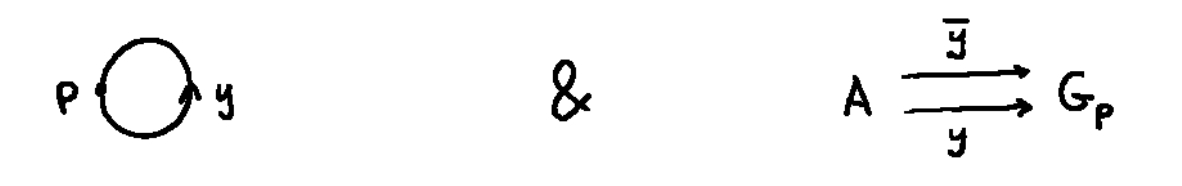
\includegraphics[width=0.5\linewidth]{sections/alicja/HNN loop and monomorphisms.jpeg}
    \caption{Graph $Y$ and monomorphisms it comes with}
    \label{loopHNN}
\end{figure}

\begin{importantexample}[\ref{HNN graph} for BS groups] In this example we will use multiplicative notation when talking about $\Z = \langle b \rangle$. 

We let $Y$ be a graph with vertex group $G_p = \Z$, and edge group $G_y = m\Z$. We set the monomorphism $a \mapsto a^y$ to be $(b^m)^k \mapsto (b^m)^k$, and this identifies $m\Z$ with its copy living inside $\Z$. We let the other morphism be $\phi: m\Z \to \Z$, $(b^m)^k \mapsto (b^n)^k$. Note, that $\phi$ is actually mapping $m\Z$ into $n\Z$ inside $\Z$. Using that observation, the fundamental group of $Y$ is $\Z \ast _\phi$, which by \ref{BS as HNN} is the group $BS(m,n)$.
\end{importantexample}

The next construction will be based on \cite[pages 23-24]{GoPaXi24}, cross-referenced with \cite{BajoHNN} where less general case is provided.

\begin{construction}
    Let $\mathbb{X} = (G,Y)$ be a graph of groups, with underlying graph $Y$ and fundamental group $\pi = \pi_1(G,Y,T)$, where $T$ is a maximal tree of $Y$.
    The Bass-Serre tree $\Tilde{X}$ of $\mathbb{X}$ is constructed as follows:
    \begin{itemize}
        \item it has vertices $vert \: \Tilde{X} = \{\pi/G_x\:|\: x \in vert\:Y\}$, and
        \item its edges are $edge \: \Tilde{X} = \{\pi/G_y \: | \: y \in edge \:Y \}$, where
        \item for each $gG_y$, $o(gG_y)) = gG_{o(y)}$ and $t(gG_y) = gyG_{t(y)}$.
    \end{itemize}
\end{construction}

Having stated the construction, two questions should come to mind, namely - why is this a connected graph and moreover, a tree. Instead of addressing those, we will see what this construction gives for $BS(m,n)$, and hopefully believe the resulting graph is indeed a tree.

\begin{example}
    To construct the Bass-Serre tree of $BS(m,n)$ \textcolor{red}{continue this}
\end{example}



